{\bf 2026-09-30}
I have a simple simulation pipeline that can make a toast simulation scanning a custom map, with or without pointing jitter. Then run a ml mapmaker or a filter bin mapmaker on the resulting TOD. 

The input map looks like this - for a 10arcmin source:

\begin{figure}[h!]
    \centering
    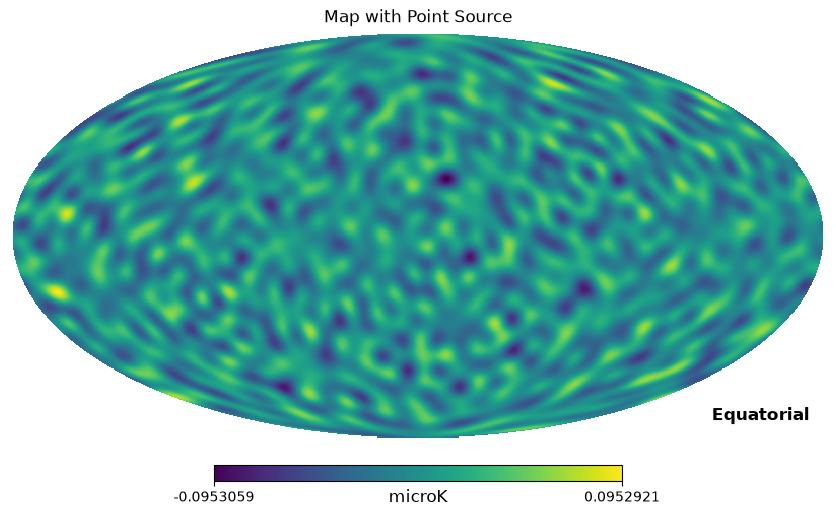
\includegraphics[width=0.75\textwidth]{figures/simple_map_wsource.png}
    \caption{Input map for the simulation.}
    \label{fig:input_map}
\end{figure}

\begin{figure}[h!]
    \centering
    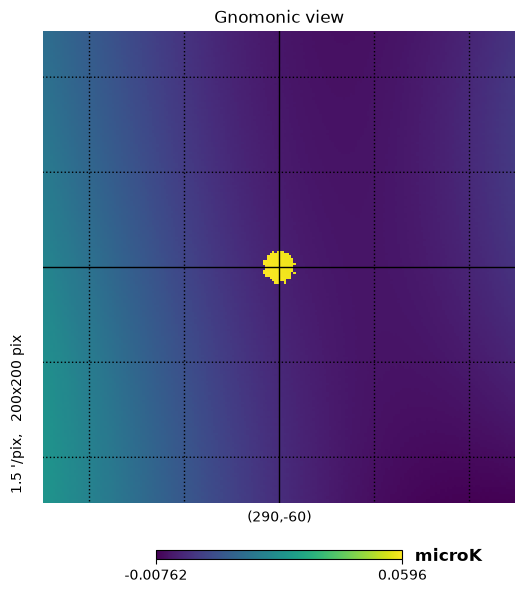
\includegraphics[width=0.75\textwidth]{figures/simple_map_wsource_gnom.png}
    \caption{Input map for the simulation - gnomonic projection of the source.}
    \label{fig:input_map_gnom}
\end{figure}


The toast sim also produces some pointing visualizations to confirm that the pointing jitter is being applied as expected.

\begin{figure}[h!]
    \centering
    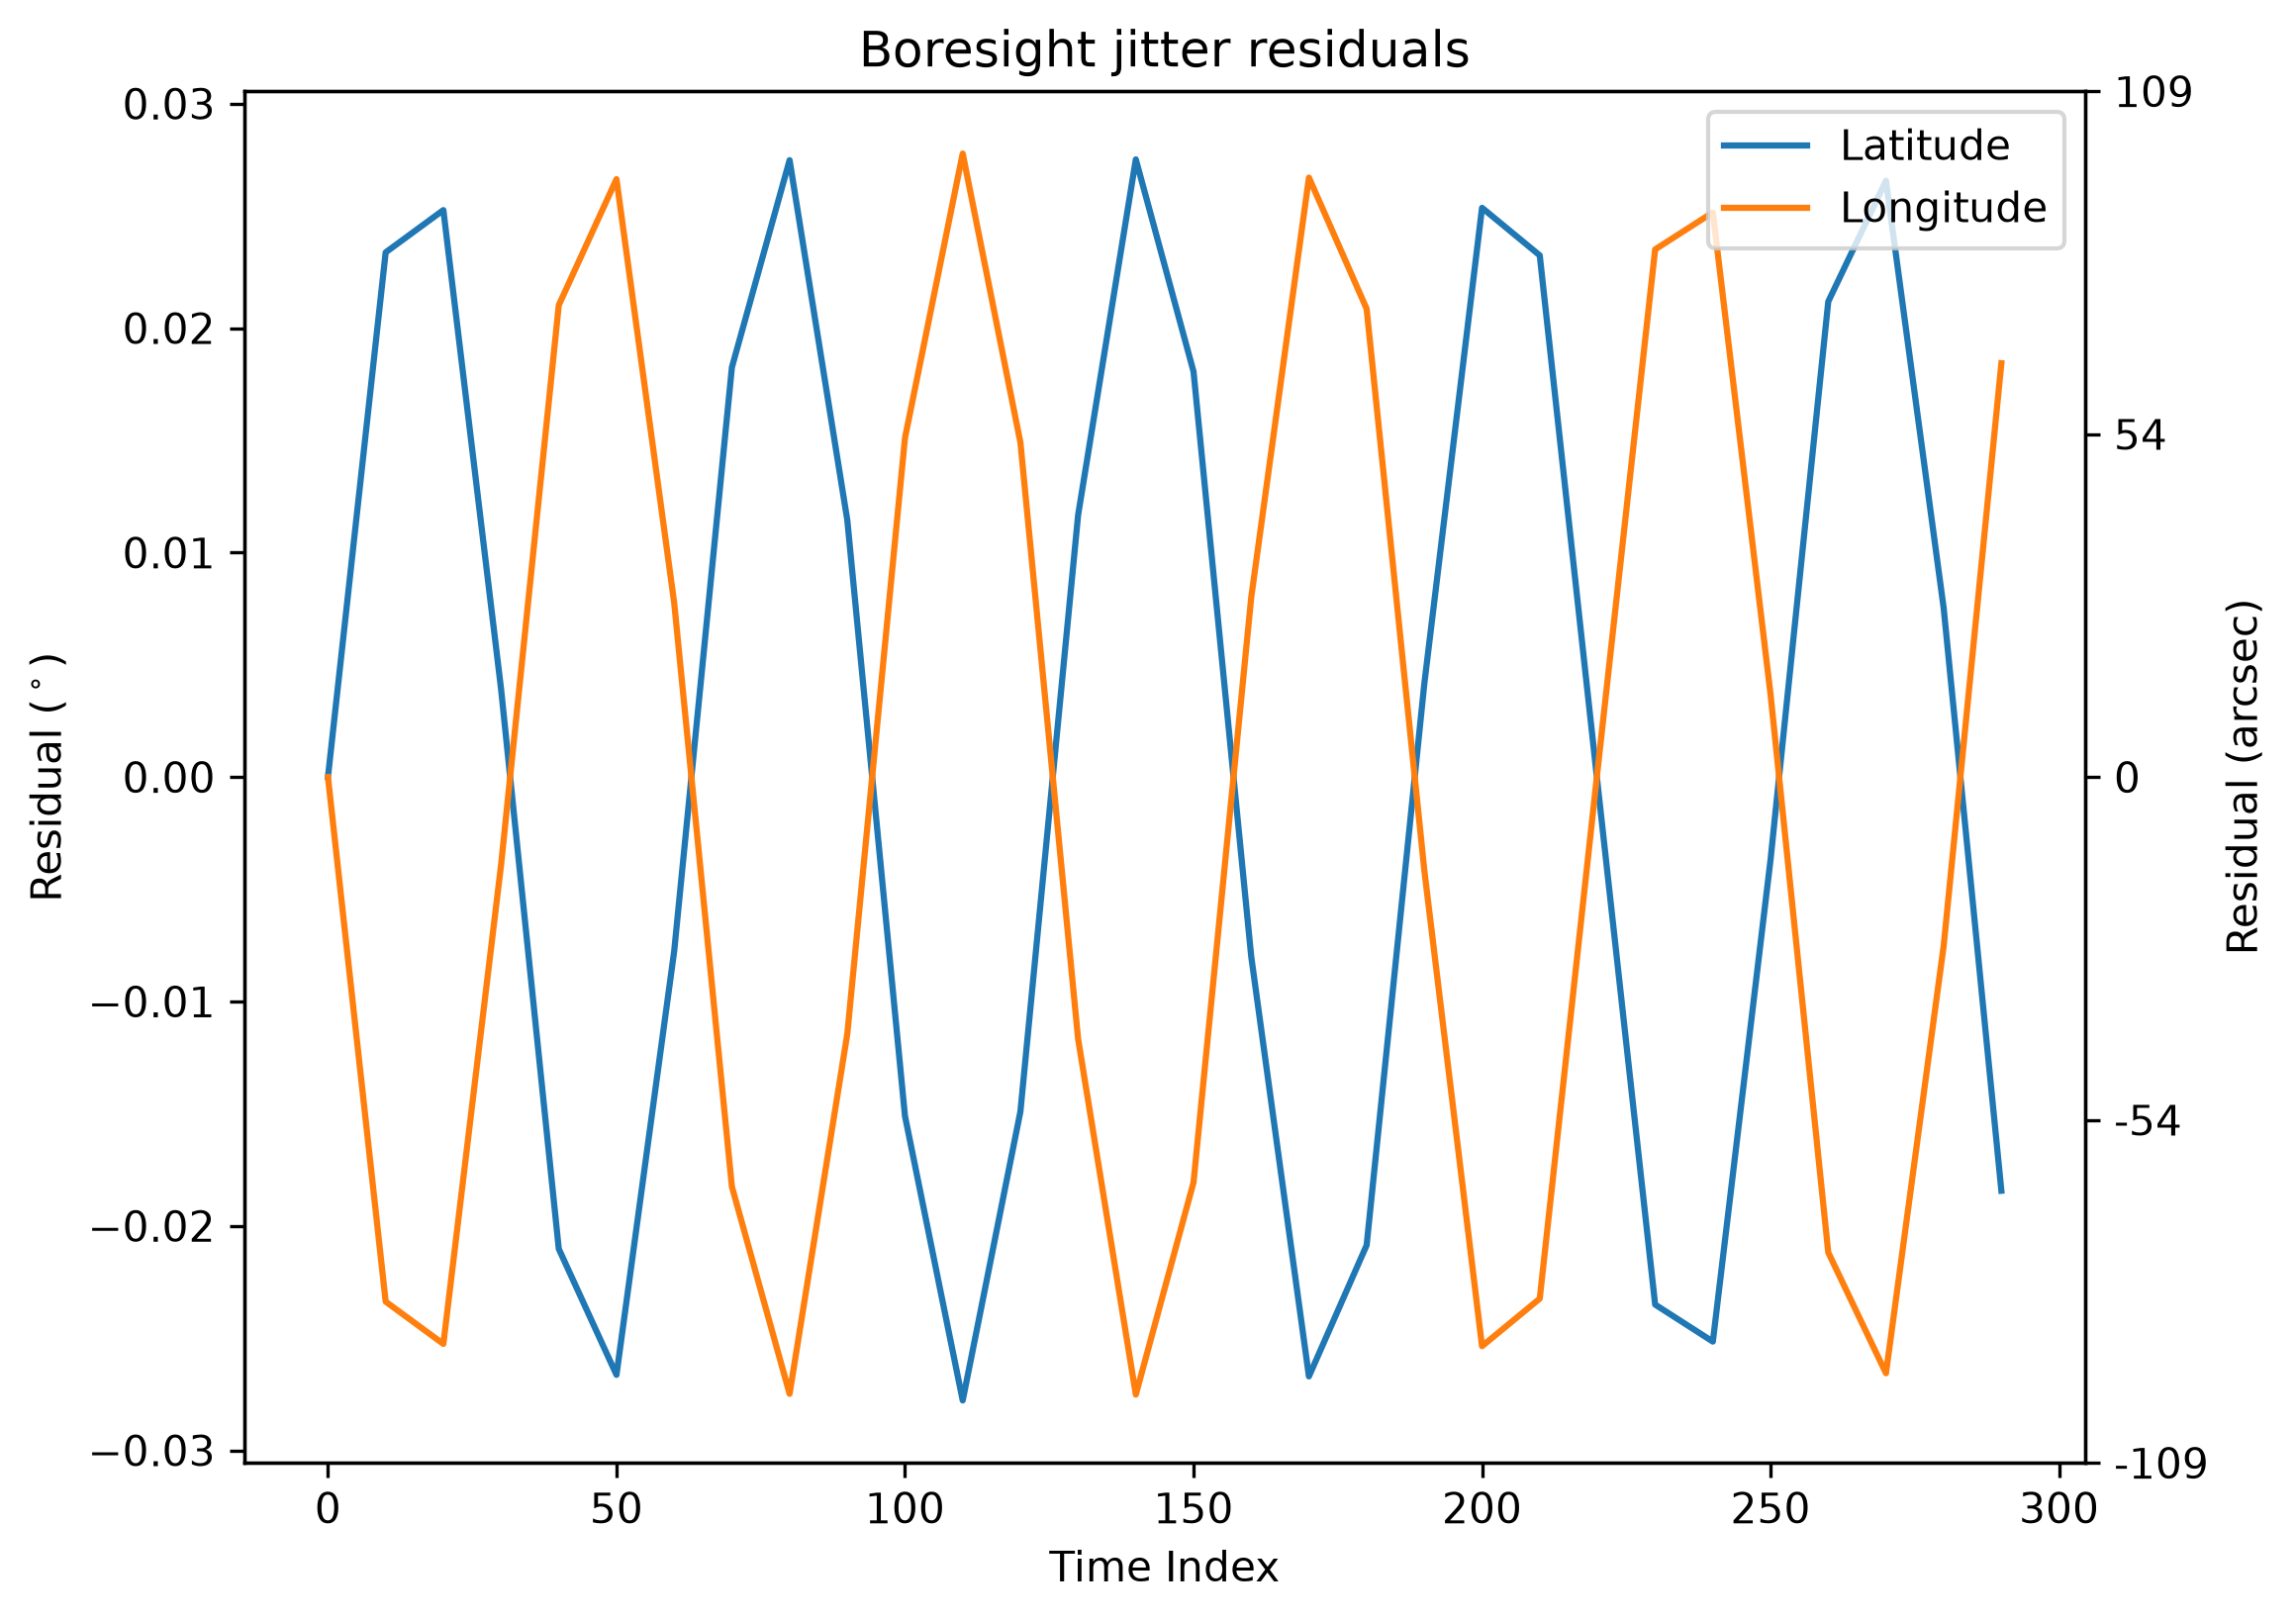
\includegraphics[width=0.75\textwidth]{figures/boresight_residuals.png}
    \caption{Pointing jitter boresight residuals.}
    \label{fig:boresight_res}
\end{figure}

After the ml mapmaker, the resulting map look like:

\begin{figure}[h!]
    \centering
    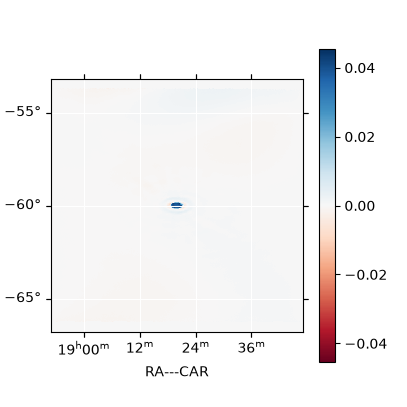
\includegraphics[width=0.75\textwidth]{figures/simple_nojitter_mlmap_I.png}
    \caption{Output I map of ML mapmaker with no jitter.}
    \label{fig:mlmap}
\end{figure}